\documentclass[a4paper]{article}
\usepackage[utf8]{inputenc}
\usepackage[russian]{babel}
\usepackage{float}
\usepackage{graphicx}
\usepackage{amsmath}
\usepackage{amssymb}
\usepackage{amsthm}
\usepackage[unicode, pdfborder = {0 0 0}, colorlinks, linkcolor = black]{hyperref}
\usepackage[raggedright]{titlesec}
\usepackage{mathtools}


\DeclarePairedDelimiter\ceil{\lceil}{\rceil}
\DeclarePairedDelimiter\floor{\lfloor}{\rfloor}


\titleformat{\chapter}[block]
  {\normalfont\huge\bfseries}{\thechapter}{20pt}{}
\titlespacing*{\chapter}
  {0pt}{20pt}{20pt}

\setcounter{tocdepth}{5}
\setcounter{secnumdepth}{5}


\parindent = 7mm
\oddsidemargin = 5mm
\topmargin = -10mm
\textheight = 240mm
\textwidth = 165mm
\linespread{1.5}


\renewcommand{\small}{\fontsize{12}{14.5pt}\selectfont}
\renewcommand{\normalsize}{\fontsize{14}{16pt}\selectfont}
\renewcommand{\large}{\fontsize{17}{20pt}\selectfont}
\renewcommand{\Large}{\fontsize{20}{25pt}\selectfont}
\renewcommand{\LARGE}{\fontsize{25}{30pt}\selectfont}
\renewcommand\qedsymbol{$\blacksquare$}

\newtheorem{theorem}{Теорема}[section]
\theoremstyle{definition}
\newtheorem{statement}{Утверждение}[section]
\newtheorem{definition}{Определение}[section]
\newtheorem*{example}{Пример}

\newenvironment{Proof}
    {{\bf \flushleft{Доказательство.} \\}}
    {\hfill$\scriptstyle\blacksquare$}


\newcounter{qcounter}


\begin{document}
\normalsize

    \thispagestyle{empty}
    \begin{titlepage}
    \begin{center}


    \vfill
    МИНОБРНАУКИ РОССИИ\\
    \vspace*{0.3cm}
    Федеральное государственное автономное образовательное\\
    учреждение высшего образования\\
    «Южный федеральный университет»\\
    \vspace*{0.3cm}
    Институт математики, механики и компьютерных наук им.\\
    И.И.Воровича\\
    Кафедра алгебры и дискретной математики
    \vfill


    \bigskip


    {\large\bf Ковалев~Никита~Евгеньевич}
    \vfill
    {\large\bf ВОССТАНОВЛЕНИЕ ЦИФРОВЫХ ИЗОБРАЖЕНИЙ\\
               С ВЫРОЖДЕННЫМ СМАЗОМ}

\fontsize{14}{16pt}\selectfont

    \vfill
    ВЫПУСКНАЯ КВАЛИФИКАЦИОННАЯ\\ РАБОТА БАКАЛАВРА\\
    по направлению 01.03.02 — Прикладная математика и информатика
    \vfill

    {\bf Научный руководитель~---\\
         доц., к.ф.-м.н. Козак Анатолий Всеволодович}



    \vfill

    \end{center}

    \bigskip

    \begin{center}
        Ростов-на-Дону~---~2018
    \end{center}

    \end{titlepage}

%-------------------------------------
    \tableofcontents
    \newpage
%-------------------------------------


    \section{Введение}


    В данной работе рассматривается явление горизонтального циклического смаза. Само являение возникает при съемке местности с помощью вращающейся камеры при создании панорманых снимков. При возникновении этого явления смазанное изображение содержит большое количество искаженной (потерянной) информации, соответственно, появляется необходимость восстановить эти данные.


    Поскольку задача актуальна для таких областей, как военная разведка, картография, геодезия, моделирование объектов местности и других, то отснять материал заново зачастую невозможно. В силу этой специфики задача восстановления искаженных снимков приобретает наиважнейший характер.


%-------------------------------------
    \newpage
%-------------------------------------

    \section{Вспомогательные понятия}


    Введем некоторые обозначения и базовые понятия, которые будут использоваться в дальнейшем.
\vspace*{0.3cm}


    \begin{definition}
    \label{blur matrix}
	\emph{Матрицей горизонтального циклического смаза} (далее - \emph{матрицей смаза}) на $k$ пикселей называется матрица $C(n, k) \in M_n$ вида
    $$
    C(n, k) = \frac{1}{k}\begin{pmatrix}
          \overbrace{1 \hspace*{2mm} \ldots \hspace*{2mm} 1 \hspace*{2mm} 1}^{k} \hspace*{2mm} 0 \hspace*{2mm} \ldots \hspace*{2mm} 0 \\
          0 \hspace*{2mm} 1 \hspace*{2mm} \ldots \hspace*{2mm} 1 \hspace*{2mm} 1 \hspace*{2mm} \ldots \hspace*{2mm} 0 \\
          \ldots \hspace*{2mm} \ddots \hspace*{2mm} \ldots \hspace*{2mm} \ddots \hspace*{2mm} \ldots \\
          1 \hspace*{2mm} \ldots \hspace*{2mm} 0 \hspace*{2mm} 1 \hspace*{2mm} 1 \hspace*{2mm} \ldots \hspace*{2mm} 1 \\
          \ldots \hspace*{2mm} \ddots \hspace*{2mm} \ldots \hspace*{2mm} \ddots \hspace*{2mm} \ldots\\
          \underbrace{1 \hspace*{2mm} \ldots \hspace*{2mm} 1}_{k-1} \hspace*{2mm} 0 \hspace*{2mm} 0 \hspace*{2mm} \ldots \hspace*{2mm} 1
        \end{pmatrix}
    $$
    \end{definition}


    В дальнейшем будем отождествлять понятие матрицы смаза и обозначения $C(n, k)$ и просто $C$ (если параметры $n$ и $k$ ясны из контекста).
\vspace{0.3cm}


    \begin{definition}
    \label{blur}
	\emph{Горизонтальным циклическим смазом} (далее - \emph{смазом}) будем называть умножение изображения на соответствующую матрицу смаза справа.
    \end{definition}


    \begin{statement}[об обратимости матрицы смаза]
    \label{inverse}
	Матрица смаза обратима тогда и только тогда, когда НОД$(n, k) = 1$.
    \end{statement}


    Следствием \ref{inverse} является, среди прочего, большее количество изображений с вырожденным смазом, нежели с невырожденным, что лишний раз подтверждает актуальность поставленной задачи.

\newpage

    \begin{example}
    Приведем пример изображений и их смазанные варианты.

\begin{minipage}{70mm}
    \begin{figure}[H]
            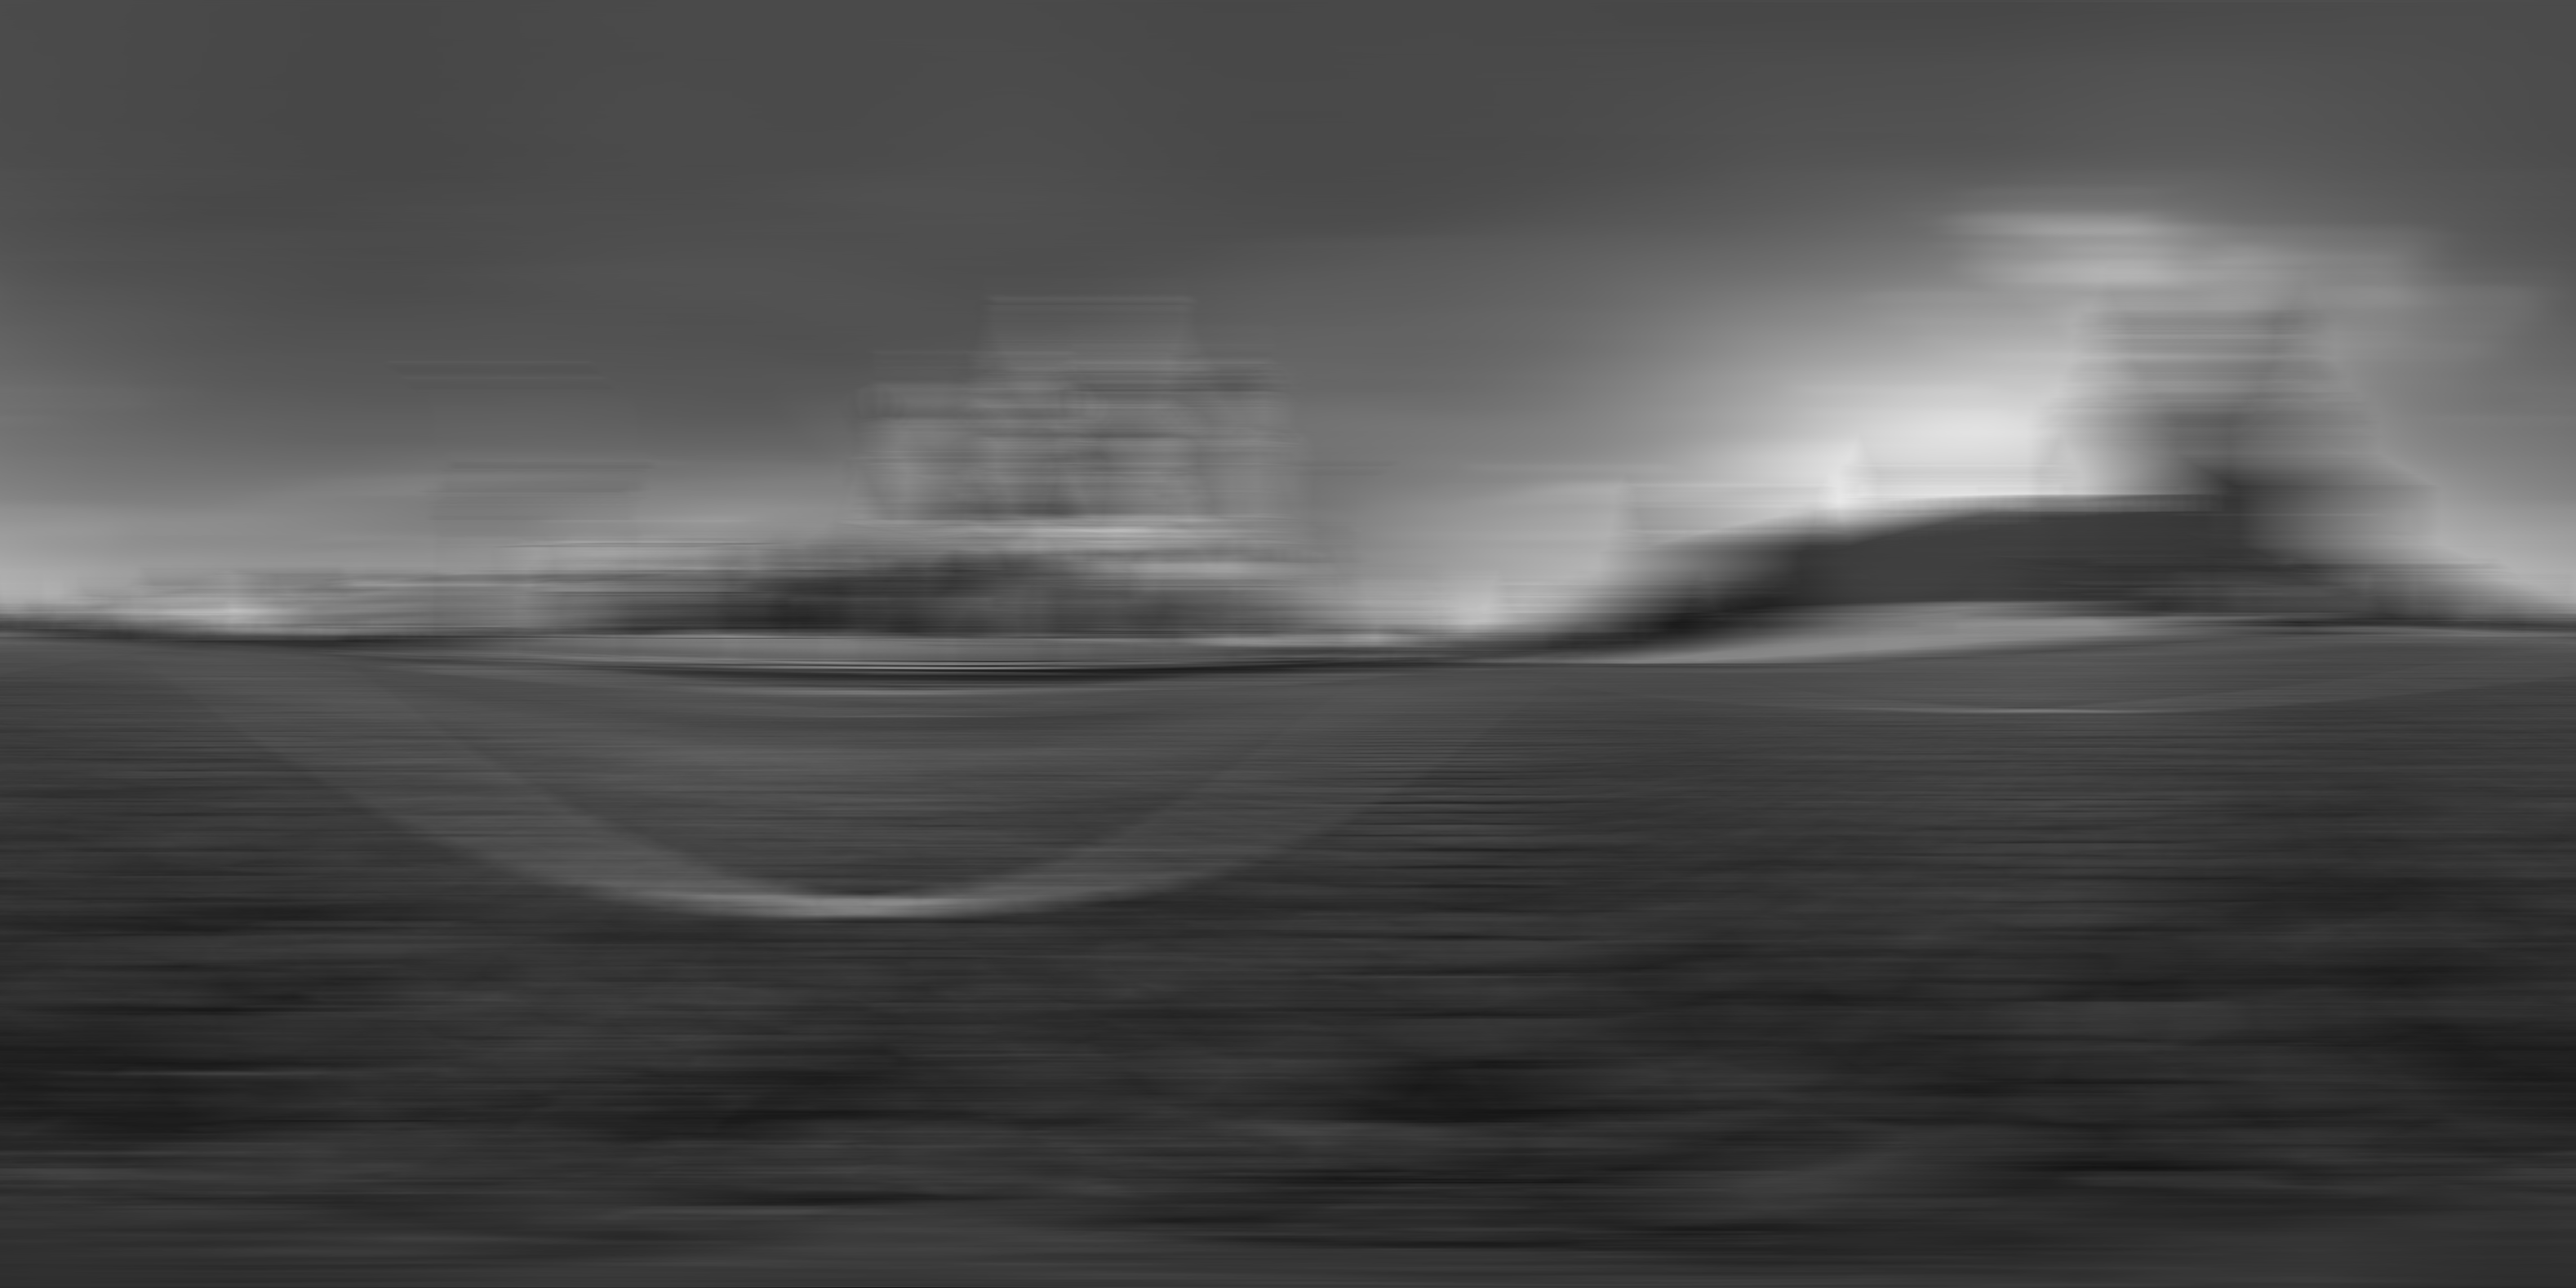
\includegraphics[scale=0.06]{D:/Diploma/Pictures/fig1.png}
            \label{Fig1}
            \caption[Смаз при $k$ = 248]{Смаз при $k$ = 248}
        \end{figure}
\end{minipage}
\hfill
\begin{minipage}{70mm}
  \begin{figure}[H]
            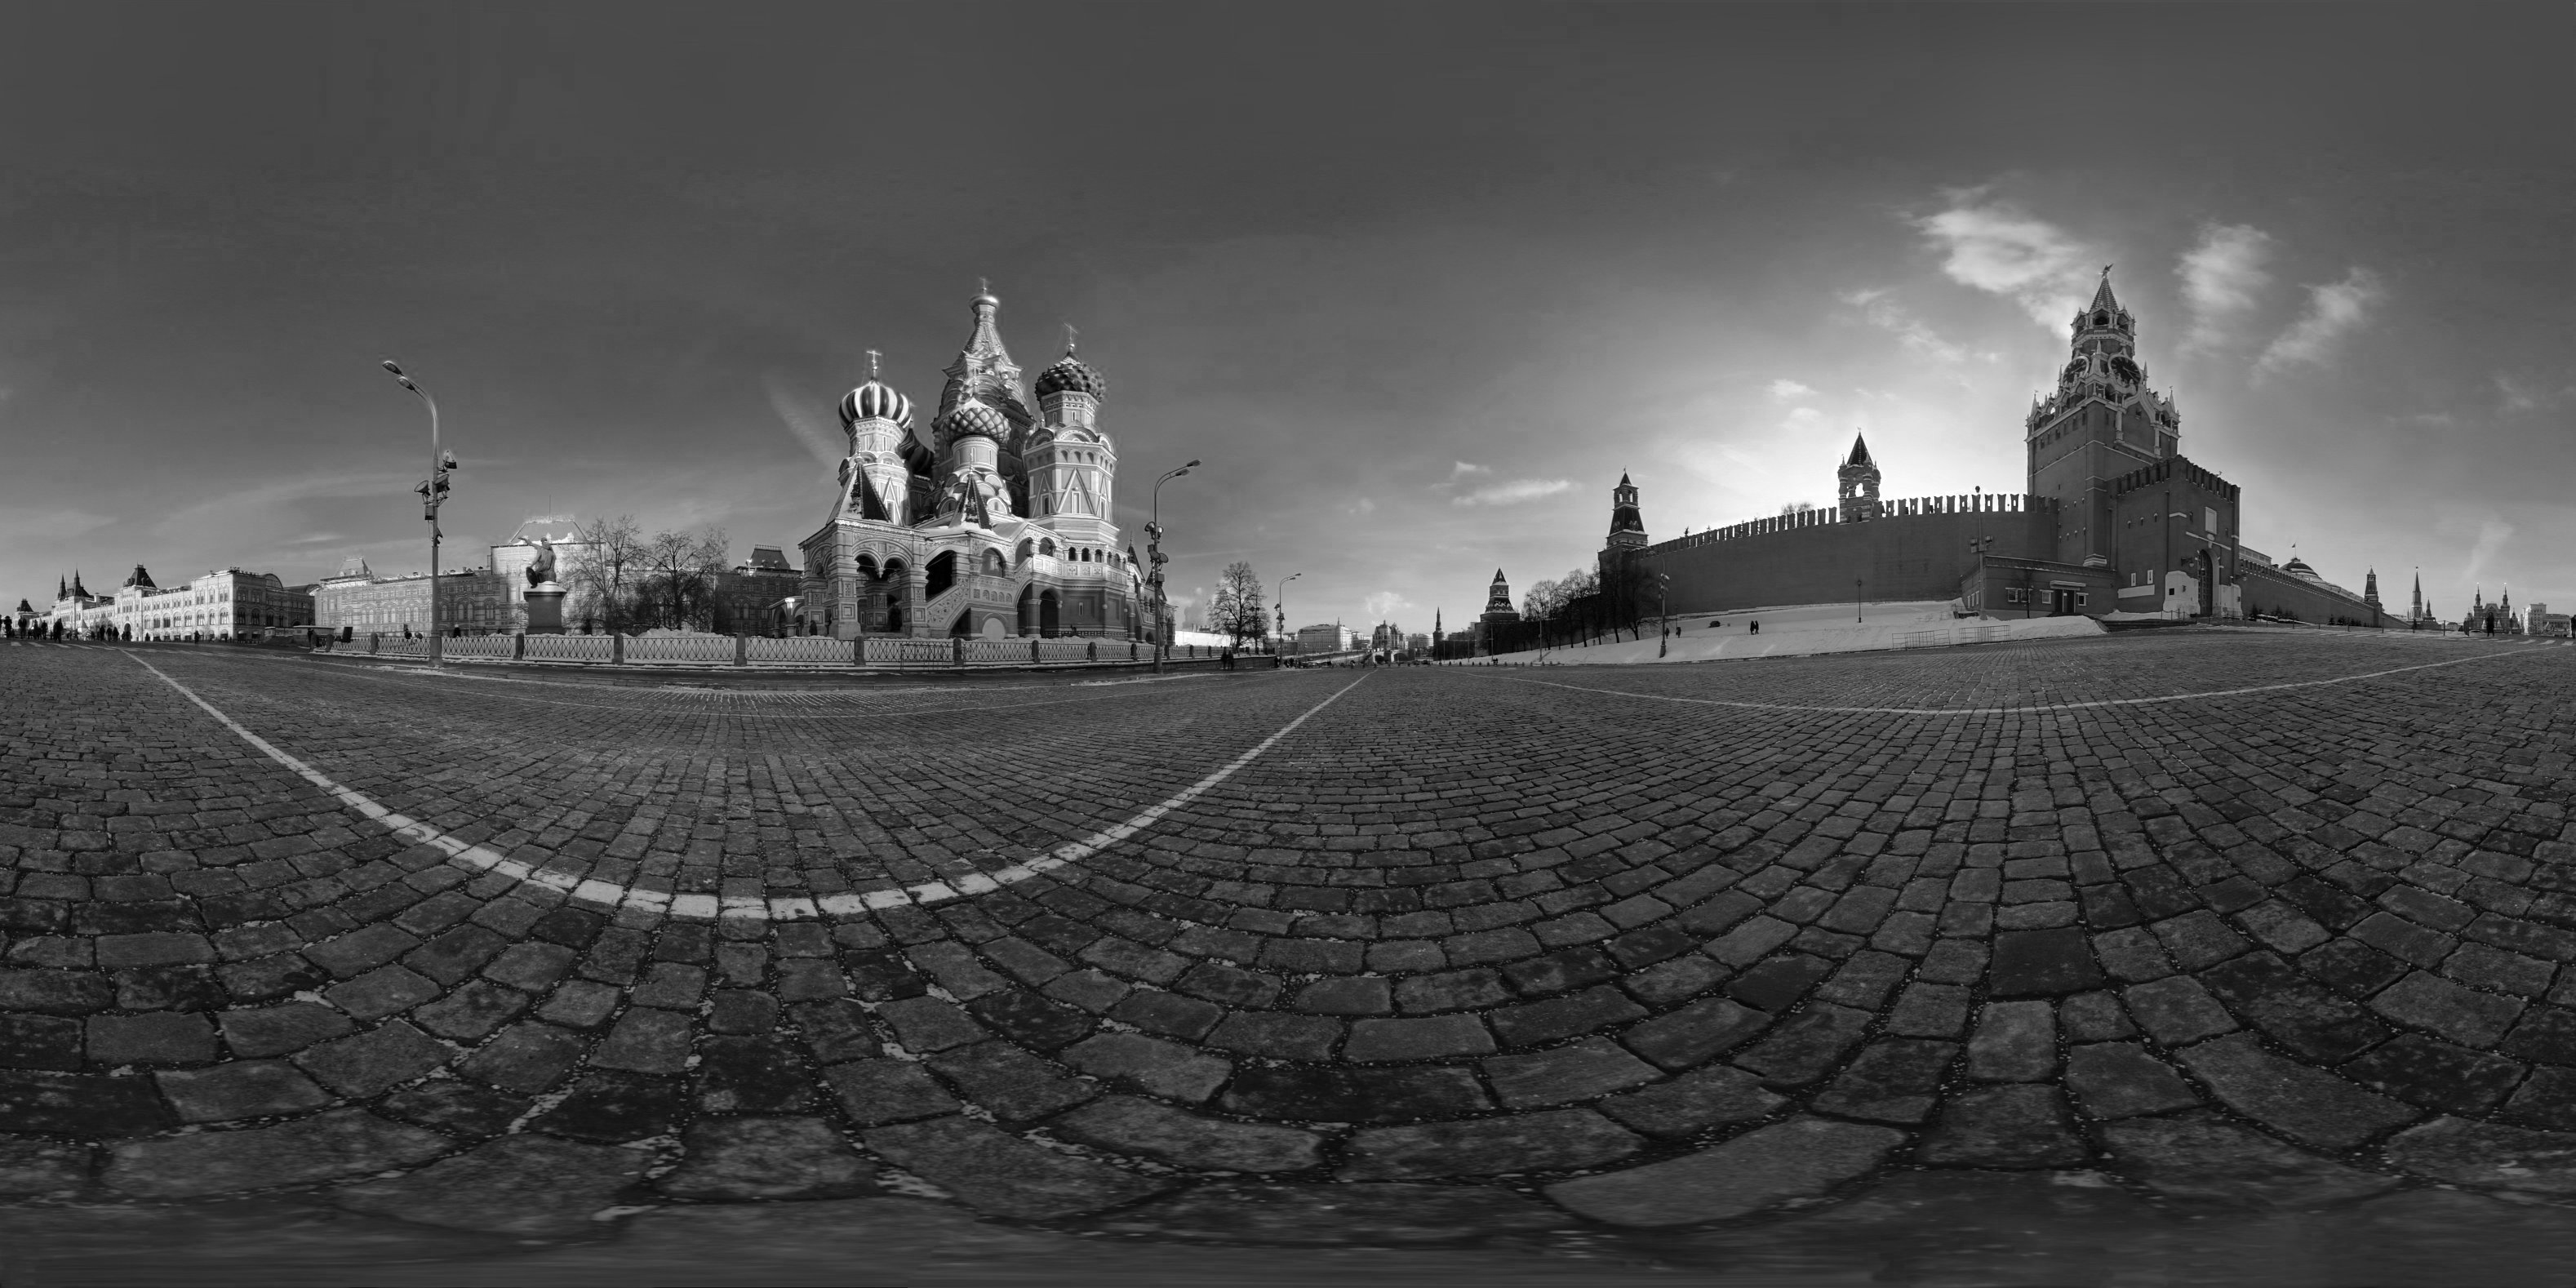
\includegraphics[scale=0.06]{D:/Diploma/Pictures/fig2.png}
            \label{Fig2}
            \caption[Исходное изображение]{Исходное изображение}
        \end{figure}
\end{minipage}
\hfill

    \end{example}

%--------------------------------------
    \newpage
%-------------------------------------


    \section{Метод предобработки в случае большого числа смаза}


    В первом параграфе пойдет речь о методе, который эффективен только для восстановления 16-битных изображений, поскольку данный подход использует обычное восстановление для невырожденного случая, а оно эффективно только для 16-битных изображений. В силу этих ограничений метод интересен не столько своей практической пригодностью, сколько подходом, который, возможно, применим в комбинации с лучшим методом восстановления.


    Подход заключается в следующем: в случае вырожденного смаза имеем $d =$ НОД$(n, k) > 1$, где $k$ - число смаза, $n$ - ширина изображения в пискелях. Тогда поделим исходное изображение $I$ на $d$ подизображений, каждое из которых содержит $i$-й столбец и далее каждый столбец, на $d$ правее предыдущего выбранного. В итоге получим последовательность $\{I_j\}_{j=1}^{d}$, каждое изображение которой содержит $\frac{n}{d}$ пискелей в ширину. Однако, каждое из этих изображений будет содержать смаз уже не на $k$, а на $\frac{k}{d}$, и, так как $d =$ НОД$(n, k)$, то НОД$(\frac{n}{d}, \frac{k}{d}) = 1$, следовательно, смаз невырожденный. Восстанавливая $I_j$ и объединяя их по тому же принципу, по какому происходило и разделение, мы получим изображение, содержащее смаз на $d$ пикселей. Объясняется это тем, что каждая из восстановленных картинок предоставляет $\frac{1}{d}$ информации от необходимой, но информация разных частей не является уникальной - все они несут примерно одну и ту же информацию. Это подтверждается экспериментально на реальных примерах.

\newpage

\begin{example}

Ниже можно увидеть пример, когда НОД двух параметров больше единицы, но незначительно (в данном случае, 16), и в таком случае восстановление происходит досточно качественно и, возможно, даже не требует дальнейшего восстановления (в зависимости от задачи).

\begin{minipage}{70mm}
    \begin{figure}[H]
            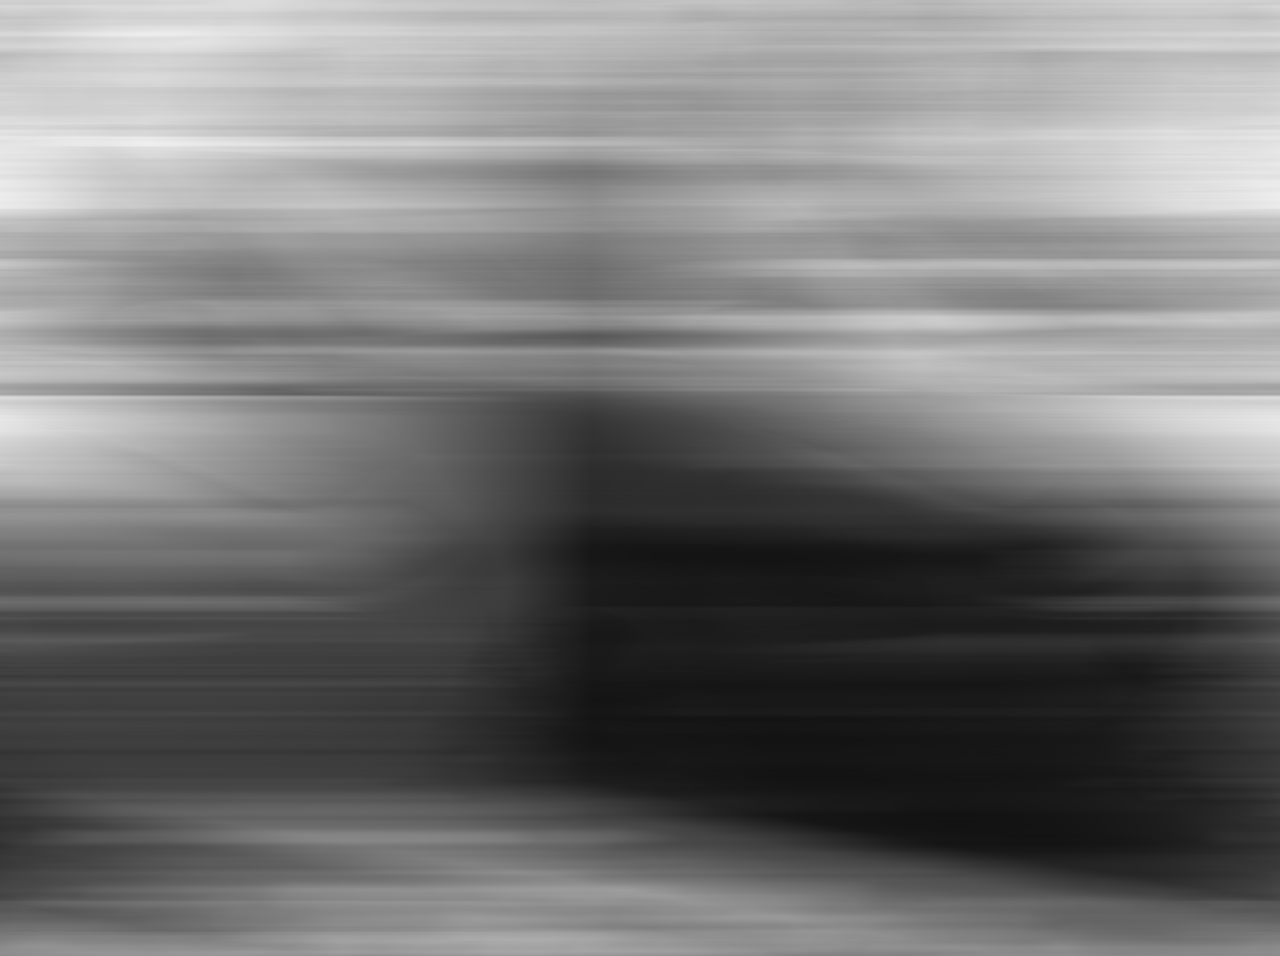
\includegraphics[scale=0.16]{D:/Diploma/Pictures/fig3.png}
            \label{Fig3}
            \caption[Смаз при $k$ = 592]{Смаз при $k$ = 592}
        \end{figure}
\end{minipage}
\hfill
\begin{minipage}{70mm}
  \begin{figure}[H]
            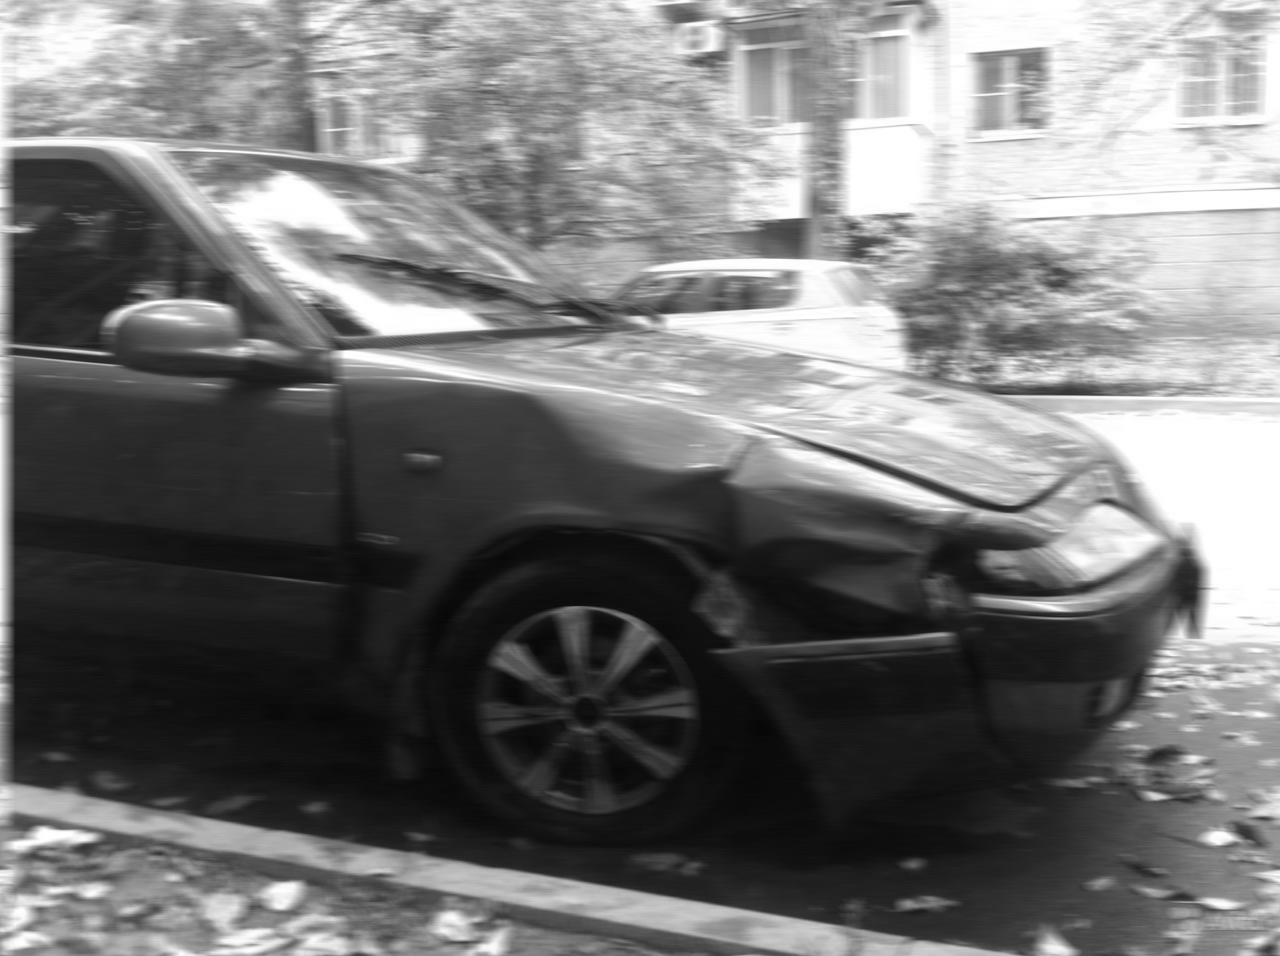
\includegraphics[scale=0.16]{D:/Diploma/Pictures/fig4.png}
            \label{Fig4}
            \caption[Улучшенное фото]{Улучшенное фото}
        \end{figure}
\end{minipage}
\hfill

\end{example}

\begin{example}

Второй пример показывает, что метод действительно работает плохо для 8-битных изображений. Тем не менее, хотя на данный момент преимущественно именно такой формат используется в фотокамерах, уже существует техника, которая сохраняет фото в 12-битном формате, и скоро получится внедрить и 16-битный формат, что позволит использовать данный метод в полном объеме, поскольку он быстрее любого другого за счет деления проблемы на подзадачи меньшего размера.

\end{example}


%--------------------------------------
    \newpage
%-------------------------------------


    \section{Метод минимизации погрешности}

    \subsection{Описание проблемы}


    Больший интерес представляют методы, которые позволяют избавиться от смаза полностью. Учитывая специфику уравнения смаза $XC = S$, где~$X$~-~исходное~изображение, $C$~-~матрица~смаза и~$S$~-~смазанное~изображение, получим, что для идеального математически восстановления необходимо найти обратную к $C$ матрицу и домножить на нее справа. Конечно, на практике это либо дает плохой результат (случай невырожденного смаза), либо невозможно (случай вырожденного смаза) в силу особенностей задачи, а именно, матрицы смаза.


    Первым препятствием является тот факт, что матрица смаза необратима при НОД$(n, k) = 1$, где $k$~-~число~смаза. Это означает, что в этом случае мы можем получить только приближенно-обратную матрицу, то есть такую матрицу $\tilde{C}$, что $C\tilde{C} \approx E$. Вторым ограничением является формат данных, с которым приходится работать при обработке изображений. В момент получения кадра изображение оцифровывается~---~непрерывная картина из окружающего мира приближается сеткой из пикселей, а значение каждого пикселя (интесивности цвета в точке) в свою очередь округляется до ближайшего целого. Таким образом, уже на данном этапе происхоит потеря огромного количества информации за счет погрешности округления.


    *здесь будут примеры восстановления в невырожденном случае и восстановления для 8 и 16 бит одного и того же изображения для иллюстрации обоих ограничений*


    Имея в виду вышесказанное, необходимо сконструировать матрицу так, что при умножении на матрицу смаза справа она дает приближение единичной матрицы~---~это даст сохранение результата, максимально приближенного к исходному теоретически, а также учесть уже имеющуюся погрешность округления и минимизировать погрешность вычислений.


    \subsection{Возможные пути решения}


    Известно, что матрица смаза представима в виде $C = FDF^{-1}$, где $D$~-~диагональная матрица, причем на диагонали~-~собственные числа матрицы $C$, а $F$~-~дискретное преобразование Фурье соотвтетствующего размера. Понятно, что в случае, когда матрица полного ранга, ее обратная находится обращением всех чисел на диагонали. Будем действовать по этому принципу, но с некоторыми поправками:


    \begin{list}{\arabic{qcounter})~}{\usecounter{qcounter}}
        \item Необратимость будем устранять заменой нулевых собственных чисел на некоторые числа с фиксированным модулем (модуль, так как собственные числа являются комплексными);
        \item Погрешность вычислений минизируем тем же способом~-~к ненулевым собственным числам, которые сильно малы по модулю, прибавим случайное комплексное число с тем же фиксированным модулем;
        \item Кроме того, оставшиеся достаточно малые собственные числа домножим так, чтобы по модулю они были равны фиксированному числу.
    \end{list}



    После соответствующих опреаций мы получим вместо матрицы $D^{-1}$, которая, вообще говоря, не всегда существует, некоторую матрицу $\tilde{D}$ такую, что $D\tilde{D} \approx E$ и $\tilde{C} = F\tilde{D}F^{-1}$. Рассмотрим, каким образом эти два преобразования повлияют на результат в теории и на практике. Эти результаты будут отличаться не только потому, что в реальной проблеме существуют погрешности, но так же и в силу особенностей порядка операций.


    \subsection{Особенности реализации на практике}


    В теории исходная матрица $X$ восстанавливается следующим порядком действий:

    $$S  F\tilde{D}F^{-1} = (X FDF^{-1}) F\tilde{D}F^{-1} = X FD\tilde{D}F^{-1},$$ то есть в идеализированной модели результат будет зависеть от того, насколько полученные числа на диагонали будут близки к числам, обратным к собственным. Также отдельно стоит отметить нулевые собственные числа - на что бы их не умножили, они останутся нулями, и соотвтествующие подобранные значения в матрице $\tilde{D}$ никакой роли не сыграют. На практике все выглядит немного иначе, поскольку матрица $S$ не расщепляется на составные части. Таким образом, влияние чисел, соответствующих нулевым собственным значениям, оказывается вполне реальным, поскольку итоговое приближение исходной матрицы $X$ будет выглядеть не иначе как $S (F\tilde{D}F^{-1}) = S\tilde{C}$. Соответственно, необходимо учитывать и этот фактор.


    \subsubsection{Поправка по умножению}


    Рассмотрим случай, когда сильно малых собственных значений не наблюдается. Тогда для каждого из них будет существовать некая поправка по умножению $\delta_i, i = \overline{0, n-1}$, а поправка по сложению не влияет на конечный результат. Это позвоялет нам рассматривать данный случай так же, как в теории, где внутренние преобразования Фурье взаимоуничтожаются. Обозначим $\tilde{E} = D\tilde{D}$, тогда:


    $$X = S \tilde{C} = X F\tilde{E}F^{-1},~~
    \tilde{E} = \begin{pmatrix}
          \frac{d_0}{d_0\delta_0} \hspace*{2mm} 0 \hspace*{4mm} \ldots \hspace*{10mm} 0 \\
          \hspace*{2mm} 0 \hspace*{2mm} \frac{d_1}{d_1\delta_1} \hspace*{2mm} \ldots \hspace*{10mm} 0 \\
          \ldots \hspace*{2mm} \ldots \hspace*{2mm} \ddots \hspace*{3mm} \ldots \\
          0 \hspace*{4mm} 0 \hspace*{2mm} \ldots \hspace*{2mm} \frac{d_{n-1}}{d_{n-1}\delta_{n-1}}
        \end{pmatrix} = \begin{pmatrix}
          \delta_0^{-1} \hspace*{5mm} 0 \hspace*{2mm} \ldots \hspace*{6mm} 0 \\
          \hspace*{2mm} 0 \hspace*{5mm} \delta_1^{-1} \hspace*{1mm} \ldots \hspace*{6mm} 0 \\
          \ldots \hspace*{2mm} \ldots \hspace*{2mm} \ddots \hspace*{3mm} \ldots \\
          0 \hspace*{4mm} 0 \hspace*{2mm} \ldots \hspace*{5mm} \delta_{n-1}^{-1}
        \end{pmatrix},
    $$ где $d$ - вектор собственных чисел матрицы $C$.


    Обозначим получившуюся матрицу $R = F\tilde{E}F^{-1}$. Тогда $R_{ij} = \frac{1}{n}\Sigma_{k=0}^{n-1} \delta_k^{-1} \xi^{(j-i)k}$, где $\xi$ есть первый корень из единицы степени $n$  $(e^{\frac{2\pi}{n}})$. Получим, что диагональные элементы $R$ равны между собой и равняются среднему величин обратных к поправкам по умножению, а элементы вне диагонали есть взвешенные средние $n$ различных корней из единицы. Важным замечением является тот факт, что эти корни различны для элементов на разных диагоналях, поскольку при удалении от главной диагонали угол между сосденими корнями $(\xi^{(j-i)k}$ и $\xi^{(j-i)(k+1)})$ увеличивается, и, соответственно, различные симметричные свойства теряются. Например, на первой диагонали, которая находится выше главной, "базовый" корень есть не что иное, как $\xi$, и, чтобы минимизировать элементы на этой диагонали, необходимо, чтобы вторая половина вектора поправок по умножению в точности повторяла первую ($\delta_0 = \delta_{\floor{\frac{n-1}{2}}+1}, \delta_1 = \delta_{\floor{\frac{n-1}{2}}+2}$ и т.д.), тогда как уже на второй диагонали условие для минимизации меняется на $\delta_i = -\delta_{\floor{\frac{n-1}{2}}+i+1}$. Таким образом, объединить условия для разных диагоналей не представляется возможным, даже если использовать поправки только для малого количества собственных значений. Это означает, что поправки по умножению, несмотря на то, что имеют детерминистскую природу, не позволяют достичь хорошиъ результатов.


    \subsubsection{Поправка по сложению}


    С поправкой по сложению все иначе. В теоретическом представлении задачи она позволяет лишь только осуществить псевдообращение матрицы смаза, но сами числа, которые мы прибавим, никоим образом не повлияют на результат. Следовательно, необходимо рассматривать матрицу

$\tilde{D}~=~diag(\frac{1}{d_0~+~\sigma_0},~\frac{1}{d_1~+~\sigma_1},~...,~\frac{1}{d_{n-1}~+~\sigma_{n-1}})$, где $\sigma$ - вектор значений поправки по сложению. Тогда аналогично п.3.3.1, положив $\gamma_i = d_i + \sigma_i$, $\tilde{R} = F\tilde{D}F^{-1}$, получим, что $\tilde{R}_{ij} = \frac{1}{n}\Sigma_{k=0}^{n-1} \gamma_k^{-1} \xi^{(j-i)k}$.


\end{document}






